\section{DES}
Il \emph{Data Encryption Standard} è un cifrario simmetrico che è stato lo standard per la crittografia di massa fino all'avvento dell'AES.
E' infatti il primo algoritmo che si basa sui principi di Shannon.
\begin{itemize}
    \item \emph{diffusione}: ogni carattere del cifrato dipende da tutti i caratteri del testo in chiaro
    \item \emph{confusione}: combinare testo in chiaro e chiave in modo complesso in modo che osservare il crittogramma non possa portare a separare le due sequenze
\end{itemize}
Questi principi sono importantissimi per la resistenza agli attacchi di crittoanalisi statistica.

Nasce nel 1972 quanto NBS (National Bureau of Standard) ora NIST (National Institute for Security and Technology) chiese la creazione di un algoritmo di crittografia simmetrica in modo da crearne uno standard. In particolare le richieste erano:
\begin{itemize}
    \item sicurezza basata sulla segretezza della chiave e non sul processo di cifratura e decifrazione (dovevano essere pubblici)
    \item l'algoritmo doveva essere efficiente sia in software che in hardware
    \item la sua sicurezza doveva essere certificata da terzi
\end{itemize}
Alla seconda richiesta l'IBM propose \emph{Lucifer} e lo lasciò studiare alla NSA che introdusse alcune variazioni:
\begin{itemize}
    \item la chiave da 128 bit passa a 56 bit
    \item cambia la S-box utilizzata
\end{itemize}

Finalmente nel 1977 viene accettato e reso pubblicamente disponibile (licenza d'uso gratuito). Diventa uno standard.
E' rimasto in vita fino al 1999 quando ne è stato sconsigliato l'uso per una versione più aggiornata: il 3-DES.
Nel 2005 anche il 3-DES diventa sconsigliato a fronte dell'AES proposto nel 2000 ed entrato nel 2001 all'utilizzo di massa.

Nel DES la cifratura è a blocchi di 64 bit, la chiave è di 64 bit in cui 56 sono casuali ed 8 sono di parità (ogni 7 un bit di parità).
La cifratura si compone di $r=16$ fasi in cui si ripetono le stesse operazioni. In ogni fase si sceglie una chiave detta sottochiave di fase.

\begin{wrapfigure}[28]{L}{4.75cm}
    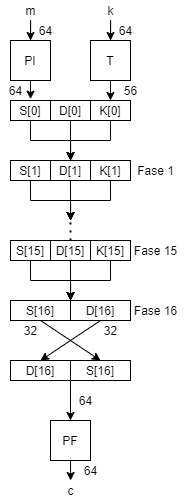
\includegraphics[width = 125pt]{DES_1.png}
\end{wrapfigure} 
I componenti sono:
\begin{itemize}
    \item m: blocco del messaggio
    \item c: corrispondente blocco del crittogramma
    \item k: chiave segreta con i bit di parità
    \item PI: permutazione iniziale (non c'è sempre)
    \item PF: permutazione finale (non c'è sempre)
\end{itemize}
Il messaggio si divide in due parti: S, D ed entrano assieme alla chiave nelle varia fasi, si esegue questo per 16 volte, alla fine si permuta se c'è bisogno e si è ottenuto il blocco.

Per decifrare si esegue lo stesso procedimento ma con le chiavi al contrario. Per ogni $i=1, 2, \_, 16$ abbiamo:
$$ S[i-1], D[i-1], K[i-1] $$
e si applicano:
$$ S[i] = D[i-1] $$
$$ D[i] = S[i-1] \oplus f(D[i-1],K[i-1]) $$

La funzione usata è \emph{non} lineare ed è detta \emph{S-box}. PI, PF e T sono delle tabella che vanno lette per riga:
\begin{itemize}
    \item PI riordina i bit di $m=m_1m_2\_m_64$ come $m_{58}m_{50}\_m_{7}$ (bit 1 va in posizione 40, il bit 58 va in posizione 1, ecc, ecc)
    \item PF è la permutazione inversa di PI (quindi riporta il bit 40 in posizione 1, ecc, ecc)
    \item T scarta i bit di parità ($k_8, k_{16}, \_, k_{64}$) e questa sequenza di 56 bit costituisce, dopo una permutazione, la chiave K[0].
\end{itemize}

La fase $i$-esima del DES è:

\begin{figure}[H]
    \centering
    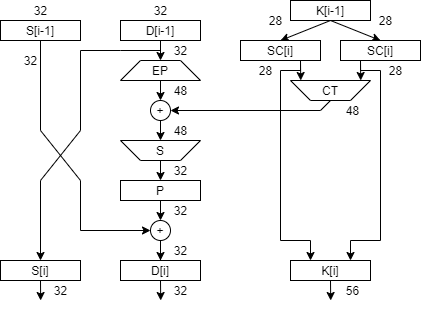
\includegraphics[width = 300pt]{DES_2.png}
\end{figure}
con:
\begin{itemize}
    \item SC: shift ciclico a sx di:
    \begin{itemize}
        \item 1 se $i \in \{1, 2, 9, 16\}$
        \item 2 altrimenti
    \end{itemize}
    \item P: permutazione
    \item EP: espansione
    \item S: S-box
    \item CT: elimina alcuni bit della chiave e li permuta
\end{itemize}

\begin{wrapfigure}{l}{4cm}
    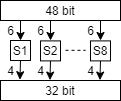
\includegraphics[width = 100pt]{DES_3.png}
\end{wrapfigure}
La S-box ha questa struttura:
Implementa 8 funzioni booleane a 6 input e a 4 output (in bit).
Si costruisce tramite la tabella di verità delle singole funzioni.

\clearpage

Queste tabelle di verità vanno però lette in una maniera particolare (di seguito la tabella di S1):
\begin{table}[ht!]
    \centering
    \small
    \begin{tabular}{c|c c c c c c c c c c c c c c c c}
        & 0 & 1 & 2 & 3 & 4 & 5 & 6 & 7 & 8 & 9 & 10 & 11 & 12 & 13 & 14 & 15 \\
        \hline
        0 & 14 & 4 & 13 & 1 & 2 & 15 & 11 & 8 & 3 & 10 & 6 & 12 & 5 & 9 & 0 & 7 \\
        1 & 0 & 15 & 7 & 4 & 14 & 2 & 13 & 1 & 10 & 6 & 12 & 11 & 9 & 5 & 3 & 8 \\
        2 & 4 & 1 & 14 & 8 & 13 & 6 & 2 & 11 & 15 & 12 & 9 & 7 & 3 & 10 & 5 & 0 \\
        3 & 15 & 12 & 8 & 2 & 4 & 9 & 1 & 7 & 5 & 11 & 3 & 14 & 10 & 0 & 6 & 13 \\
    \end{tabular}
\end{table}
supponiamo di avere 010011: prendo gli estremi 0 ed 1 ed uso quasto come indice per la riga, prendo poi i 4 bit centrali (1001) e lo uso come indice di colonna. Accedo quindi a (1, 9) $\xrightarrow{} 06$.

NB: perché è importante che non sia lineare? Perché $f(x \oplus y) \neq f(x) \oplus f(y)$ ed è cruciale ai fini del funzionamento!

\subsection{Vulnerabilità}
Siano:
$$ c = C_{DES}(m, k) $$
$$ c^{*} = C_{DES}(m', k') $$
$$ m', k' \text{ complementari di m e k} $$

Si può notare che $c^{*} = c$ perché SC sposta i bit complementati quindi EP espande bit complementati e poi c'è lo XOR che ci da un risultato uguale a quello che avremmo se non fossero complementate:
$$ \bar{m_i} \oplus \bar{K_i} = (1 \oplus m_i) \oplus (1 \oplus K_i) = m_i \oplus K_i $$
L'input alla S-box è identico! Abbiamo quindi in uscita lo stesso valore che poi verrà messo in XOR con l'altra parte del messaggio che è complementato, ci fornisce quindi il risultato complementato.

\subsection{Attacchi al DES}
Sono tutti attacchi a forza bruta:
\begin{itemize}
    \item architetture appositamente progettate per attaccare il DES e quindi velocizzare criptazione e decriptazione (con 1M\$ si costruiva una macchina che forzava il DES in 35 minuti)
    \item distribuire lo spazio delle chiavi tra più utenti, è più economico e la velocità dipende da quanti utenti ci lavorano
\end{itemize}

Nel 1997 la compagnia RSA lancia una sfida: in 5 mesi esplorando il 25\% delle chiavi viene risolta la sfida e trovata la chiave.
Nel 1998 ce ne vollero 39 di giorni esplorando 85\% delle chiavi.

Qualche parola su questi attacchi: le chiavi possibili sono $2^{56}$, 64 di queste chiavi sono rimosse perché con regolarità. Ricordando che:
$$ C(m, k) = c = \bar{c} = C(\bar{m}, \bar{k}) $$
si possono dimezzare le chiavi passando a $2^{55}$ (55 bit di sicurezza). Questo è un tipo di attacco chosen plain-text in cui ci si procura delle coppie $<m, c_1>$, $<\bar{m}, c_2>$. Si inizia ad esplorare le chiavi e per ognuna si controlla:
\begin{itemize}
    \item C(m, k) = $c_1$: k POTREBBE ESSERE la chiave
    \item C(m, k) = $\bar{c_2}$: $\bar{k}$ POTREBBE essere la chiave
    
    NB: $C(m,k) = \bar{c_2} \iff C(\bar{m},\bar{k}) = \bar{\bar{c_2}} = c_2$ in quanto sappiamo che $C(m, k) = c$ e $C(\bar{m}, \bar{k})=\bar{c}$. Escludo quindi due chiavi alla volta.
    \item $\neq c_1, \bar{c_2}$: si prova un'altra chiave (k e $\bar{k}$ non lo sono)
\end{itemize}

Nel 1990 sono stati scoperti attacchi di \emph{crittoanalisi differenziale} (da Bihan e Shamir). E' un attacco di tipo chosen plain-text in cui ci si procura $2^{47}$ coppie $<m,c>$.
Si cerca tra i messaggi simili le similitudini nei crittogrammi e si sfruttano per trovare la chiave.
Si assegnano delle probabilità alle singole chiavi, ed emerge poi quella più probabile.
Dato che le fasi sono 16 si ha un costo di questo attacco pari a $2^{55.1}$, poco più di una ricerca esaustiva.

NB: se fosse $r=8$ si avrebbe difficoltà $2^{14}$

Nel 1993 sono stati scoperti attacchi di \emph{crittoanalisi lineare} che consistono nella costruzione di una approssimazione lineare della S-box che ci permette di inferire taluni bit della chiave, il resto si bruta.
Si scende a $2^{43}$ coppie $<m, c>$ ed è di tipo known plain-text.
Metodo più efficiente del forza bruta.

\subsection{Varianti del DES}

\subsubsection{Scelta indipendente delle sottochiavi}
Anziché generare le sottochiavi di fase a partire dalla chiave principale si scelgono manualmente.
E' come passare da 56 bit a $16 \cdot 48 = 768$ bit di chiave.
Tuttavia non porta effettivamente ad un aumento della sicurezza perché è sempre vulnerabile ad attacchi differenziali portando a $2^{61}$ la complessità di un attacco.

\subsubsection{Cifratura multipla: 2DES}
$$ \forall k_1, k_2, k_3: C_D(C_D(m, k_1), k_2) \neq C_D(m, k_3) $$
quindi applicare due volte la cifratura DES non è uguale ad applicarlo una sola volta.
Si arriva ad uno spazio delle chiavi di $2^{112}$.
Tuttavia esiste l'attacco \emph{meet-in-the-middle} che fa scendere la sicurezza a 57 bit di chiave:
$$ c = C(C(m,k_1), k_2) $$
$$ D(c,k_2) = C(m,k_1) $$
possiamo quindi prendere una coppia $<m, c>$:
$$ \forall k_1 \text{ mi salvo } C(m, k_1) \xrightarrow{} 2^{56} \text{ cifrature }$$
$$ \forall k_2 \text{ mi calcolo } D(c, k_2) \xrightarrow{} 2^{56} \text{ cifrature al più }$$
Cercando nella lista delle cifrature, so che esisterà una coppia $<k_1, k_2>$ per la quale c'è la corrispondenza:
$$ D(c, \bar{k_2}) = C(m, \bar{k_1}) $$.

Questo attacco costa quindi $2^{56} + 2^{56} = 2 \cdot 2^{56} = 2^{57}$ al più, tra cifrature e decifrature.

\subsubsection{Cifratura multipla: 3DES}
Presente in due modi:
\begin{itemize}
    \item 2TDEA:
        $$ c = C(D(C(m, k_1), k_2), k_1) $$
        $k_1$ e $k_2$ sono chiavi di 56 bit tra di loro indipendenti. Si sceglie questa modalità perché se pongo $k_1 = k_2$ ottengo il DES normale, quindi risulta essere retrocompatibile.
        
        NB: CDC non è più robusto di CCC. Ha un livello di sicurezza di 112 bit.
    \item 3TDEA: triple data encryption algorithm
        $$ c = C(D(C(m, k_1), k_2), k_3) $$
        $k_1$, $k_2$, $k_3$ chiavi a 56 bit. Si hanno quindi chiavi di $3 \cdot 56 = 168$ bit. E' vulnerabile a meet-in-the-middle quindi la sicurezza scende a 112 bit di sicurezza.
\end{itemize}